\begin{figure}[htb]
  \centering
%segundo bloco de figuras
  \begin{tabular}{c c c c c }
    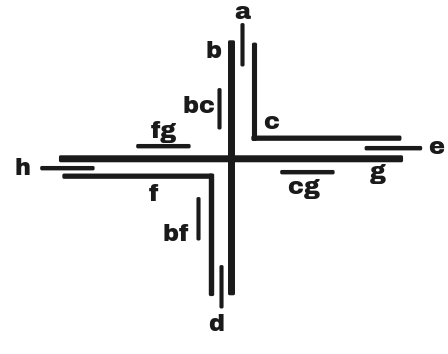
\includegraphics[width=4cm]{./img/falsePie.png}  %\label{fig:falsePie} 
    & &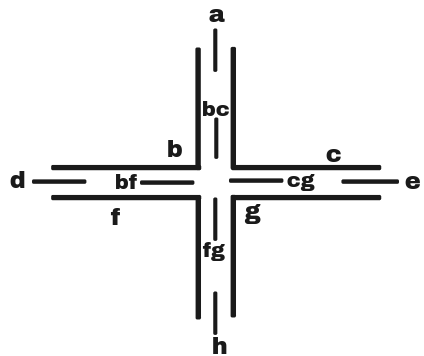
\includegraphics[width=4cm]{./img/truePie.png} %\label{fig:truePie}
    & &
 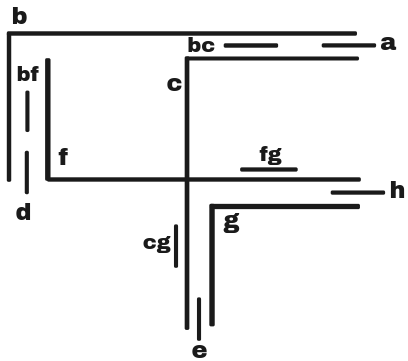
\includegraphics[width=4cm]{./img/frame.png} \\%[\abovecaptionskip]
    {\footnotesize (a) Based in false pie}  & &  {\footnotesize(b) Based in true pie} & & {\footnotesize (c) Based in frame} %\label{fig:frame}
  \end{tabular}
  \caption{Different single bend representations of the  graph $H$ using a false pie (a), a true pie (b) and a frame (c) for represent the $C_4^{H}$}\label{fig:falsepietruepieframe}
\end{figure} 